\subsection{Simulator}

Das Erarbeiten des Konzeptes des Simulators, der Implementierung und des Gebrauchs wird in diesem Kapitel festgehalten.

Nach der Nutzwertanalyse war das grundlegende Konzept klar und es konnte mit der Implementierung begonnen werden.

\subsubsection{Spezifikationen}

TODO: Was soll Simulator koennen?

\begin{table}[H]
\centering
\small
\begin{tabularx}{\textwidth}{|l|X|l|}
\hline
  \textbf{Nr.} & \textbf{Spezifikation} & \textbf{Priorität 1-3}  \\
  \hline
  1  & Der Zielknoten kann ausgewählt werden. &  2\\
  \hline
   2   & Der Roboter speichert den Graph intern.  & 1\\
  \hline
   3 & Der Roboter überprüft seine Nachbarsknoten.&1\\
  \hline
  4 & Der Roboter erkennt fehlende Linien und reagiert darauf. & 1\\
  \hline
  5 &   Der Roboter erkennt Pylonen und reagiert darauf. & 1\\
  \hline
   6  &   Der Roboter erkennt Barrieren und reagiert darauf. & 1\\
  \hline
    7 &   Der Roboter berechnet den kürzesten Weg im Graphen.& 1\\
  \hline
     8  &   Der Weg des Roboters wird im GUI angezeigt. & 1\\
  \hline
      9   &   Die Reaktionen auf die Hindernisse werden im GUI angezeigt. & 2\\
  \hline
 10   &   Die Hindernisse werden im GUI angezeigt. & 2\\
  \hline
   11   &   Die Reihenfolge der Knoten wird erkannt, als Vorbereitung, dass der Roboter, der Steuerung sagen kann, wo sich der nächste Weg befindet. & 3\\
  \hline

\end{tabularx}
\caption{Spezifikationen Simulator}
\label{table:spezifikation-simulator}
\end{table}

\subsubsection{Konzeption}

Es wurden mehrere Varianten ermittelt mit einem morphologischen Kasten, die alle die Spezifikatinen erfuellen koennen. Mit einer Nutzwertanalyse wurde die beste Variante bestimmt.

TODO BEschreib gewaehlte Variante, depending wo Kasten \& Analyse sind in Doku

Die einzelnen Taetigkeiten wurden in GitHub Issues festgehalten. Jedes Issue wurde jeweils der Person zugeordnet, die gerade daran arbeitet. So konnte koordiniert entwickelt werden.

\begin{figure}[H]
\centering
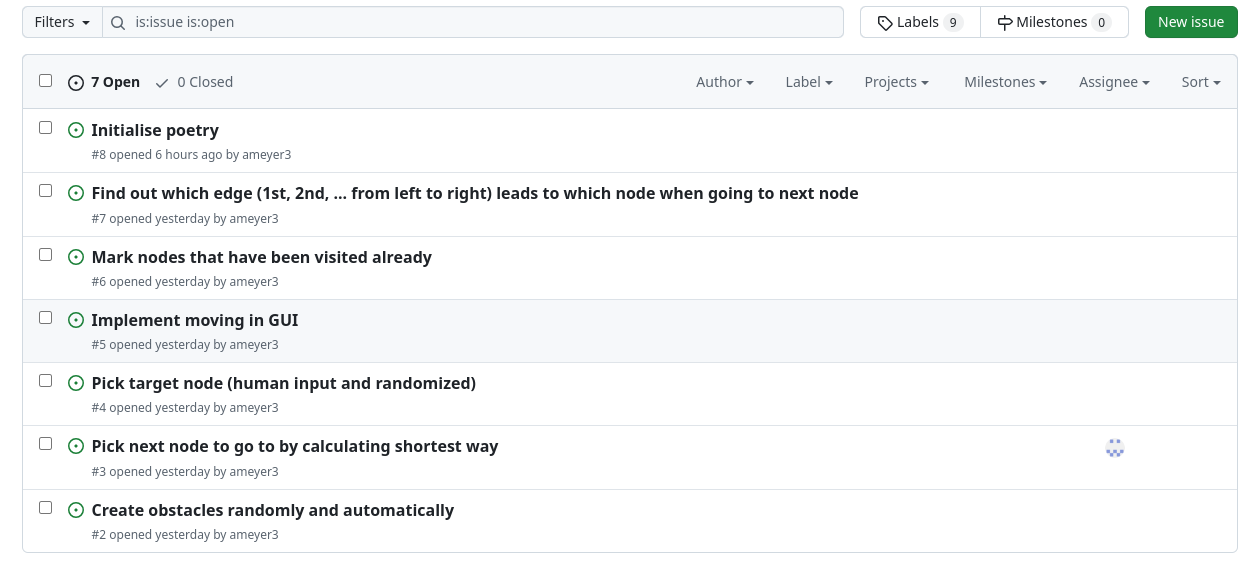
\includegraphics[width=\textwidth]{img/github-issues.png}
\caption{GitHub Issue Liste}
\label{fig:github-issues}
\end{figure}

Es wurde ein objektorientierter Ansatz gewaehlt, um den Simulator umzusetzen. Die Roboterklasse soll dabei den physischen Roboter darstellen, der die einzelnen Bauteile besitzt. So soll zum Beispiel die Wheels Klasse verwendet werden als Simulation fuer das Drehen und fortbewegen. An dieser Klasse werden diese Nachrichten gesendet, die im echten Roboter an die elektrische Steuerung gesendet werden wuerden betreffend der Fortbewegung.


\begin{figure}[H]
\centering
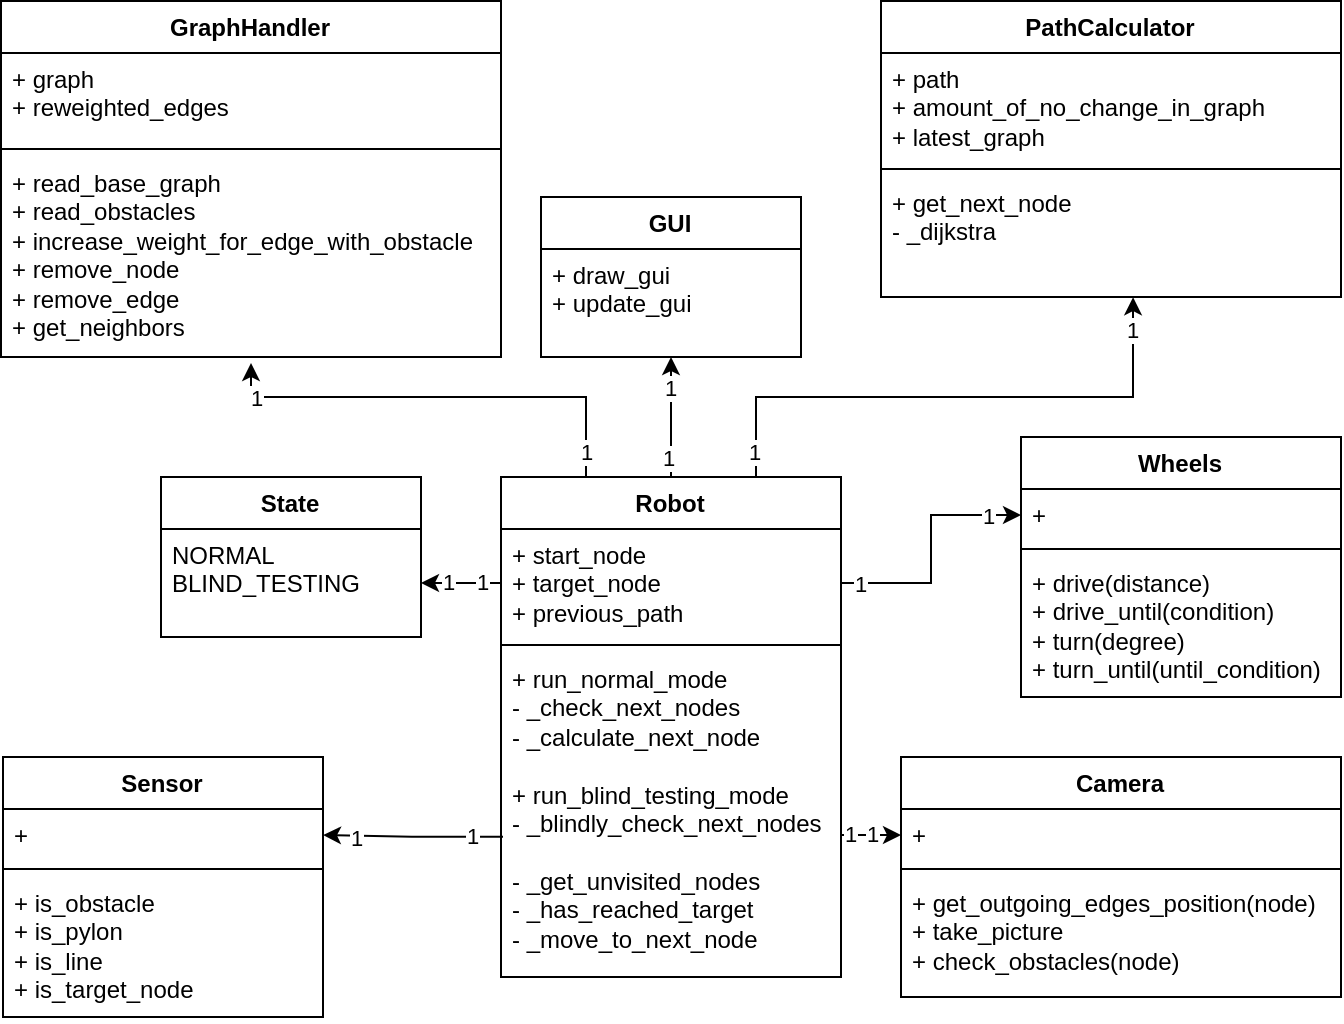
\includegraphics[width=\textwidth]{assets/informatik-prototyp/simulator/simulator-erd.png}
\caption{Simulator ERD}
\label{fig:simulator-erd}
\end{figure}

\subsubsection{Entwicklung}

Der erste Schritt war es einen Graph zu definieren. Dazu wurde ein YAML File mit dem konfigurierten Graph erstellt. 
Dazu wurde der vorgegebene Graph beschriftet: Jeder Knoten erhaelt einen Buchstaben und jede Kante ein Gewicht. Die Gewichtungen sind die relativen Laengen der Strecken. Diese Beschriftung wurde wie folgt in einem YAML File beschrieben.

\begin{figure}[H]
\begin{subfigure}{0.275\textwidth}
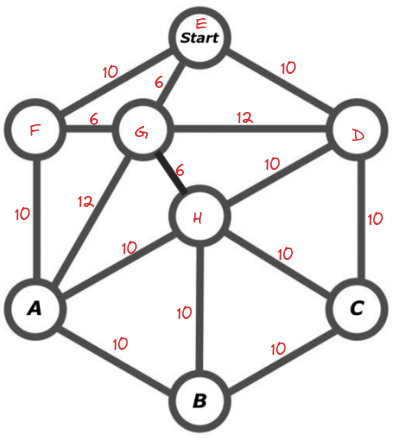
\includegraphics[width=0.95\linewidth]{img/graph_with_weighted_edges.png} 
\caption{Beschrifteter Graph}
\label{fig:labeled-graph}
\end{subfigure}
\begin{subfigure}{0.720\textwidth}
\begin{footnotesize}
\begin{verbatim}
# the edges are assorted clock-wise
A: [{ F: 10 }, { G: 12 }, { H: 10 }, { B: 10 }]
B: [{ A: 10 }, { H: 10 }, { C: 10 }]
C: [{ D: 10 }, { B: 10 }, { H: 10 }]
D: [{ E: 10 }, { C: 10 }, { H: 10 }, { G: 12 }]
E: [{ D: 10 }, { G: 6 }, { F: 10 }]
F: [{ E: 10 }, { G: 6 }, { A: 10 }]
G: [{ E: 6 }, { D: 12 }, { H: 6 }, { A: 12 }, { F: 6 }]
H: [{ G: 6 }, { D: 10 }, { C: 10 }, { B: 10 }, { A: 10 }]
\end{verbatim}
\end{footnotesize}
\caption{Graph in YAML}
\label{fig:graph-yaml}
\end{subfigure}
\end{figure}

Die Hindernisse und die fehlenden Linien sind ebenfalls in einem YAML File definiert. So koennen diese einfach angepasst werden:

\begin{verbatim}
cone:
  - F
barrier:
  - [E, G]
missing_line:
  - [E, D]
\end{verbatim}

Der Simulator liest die beiden Dateien ein und speichert sie intern als Python Dictionaries.

\textbf{Ablauf des Simulators:}

Das Ziel ist es, dass der Ablauf moeglichst nah ist an dem Ablauf des Gesamtkonzeptes.
Der Programmablauf besteht aus folgenden Teilen:
\begin{enumerate}
    \item Nachbarsknoten auf Hindernisse pruefen
    \item Naechste Knoten berechnen
    \item Zu naechstem Knoten fahren
\end{enumerate}

Es wird simuliert, dass der Roboter auf einem Knoten steht. Er dreht sich im Uhrezeigersinn im Kreis und prueft alle Nachbarsknoten. In der Simulation wird dafuer der Hindernis-Dictionary auf die jeweiligen Knoten und Strecken geprueft. Falls ein Hinderniss detektiert wirde, reagiert er wie folgt:

\begin{itemize}
    \item Ein Pylon steht auf dem Nachbarsknoten: Dieser Knoten und alle Kanten, die dahin fuehren, werden im intern gespeicherten Graph-Dictionary entfernt.
    \item Eine Barriere wird auf einer ausgehenden Strecke erkannt: Die Strecke wird im intern gespeicherten Graph-Dictionary hoeher gewichtet. TODO WIE VIEL?
    \item Eine ausgehende Linie fehlt: Diese Verbindung wird aus dem intern gespeicherten Graph entfernt.
\end{itemize}

Falls noch nie eine Berechnung des kuerzesten Weges durchgefuehrt wurde oder der intern gespeicherte Graph sich veraendert hat, wie die Berechnung der kuerzesten Pfades durchgefuehrt. Ein Dijkstra wird verwendet. Die geplante Pfad und der naechste Knoten werden gespeichert.

Danach bewegt sich der Roboter zum naechsten Knoten. Dabei wird simuliert, dass sich der Roboter zur naechsten Linie drehen soll und die Distanz zum naechsten Knoten fahren soll. Im Simulator sind alle Kanten eines Knotens im Uhrzeigersinn angeordnet gespeichert. Die Position (relativ zu der Strecke, von der der Roboter herkommt) der naechsten Strecke wird mit dem Ring Buffer Algorithmus\footnote{https://en.wikipedia.org/wiki/Circular\_buffer} berechnet. So kann Simuliert werden, dass eine Liste in einem Kreis angeordnet ist. So wird es in der richtigen Applikation moeglich sein, die Kanten zu identifizieren. 

\begin{figure}[H]
\centering
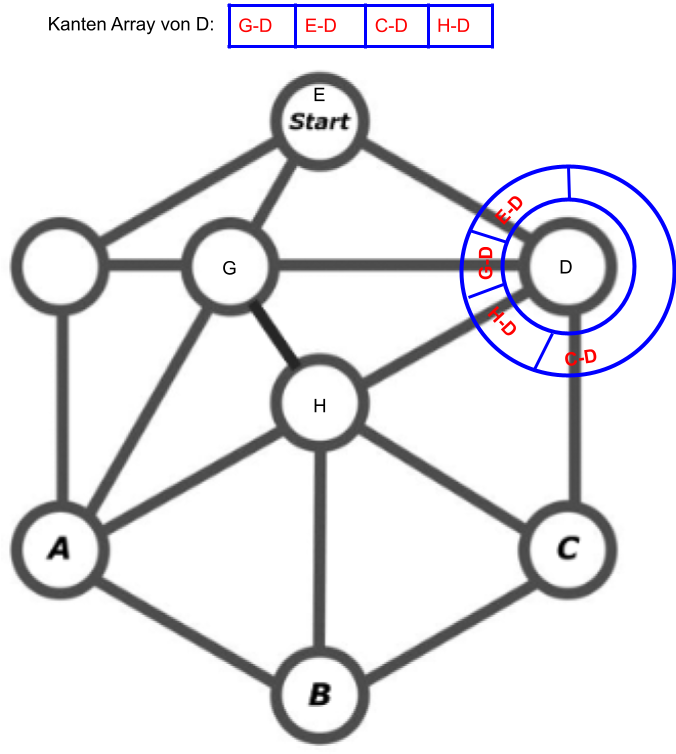
\includegraphics[width=0.75\textwidth]{assets/informatik-prototyp/simulator/ring-buffer-graph.png}
\caption{Graph with Ring Buffer}
\label{fig:ring-buffer-graph}
\end{figure}

Die Position relativ zu einer bestimmten Kante herauszufinden wird wie folgt implementiert:

\begin{verbatim}
edges_to_target = (target_index - start_index) % len(neighbors)
\end{verbatim}

Diese Ablauf wird so lange wiederholt, bis der Zielknoten erreicht wird.
Waehrend des ganzen Ablaufes werden die einzelnen Klassen aufgerufen, die die einzelnen Roboterbauteile simulieren. In diesen befindet sich zum Teil eine Mock-Logik (zum Beispiel Hindernisse aus dem Konfigurationsfile lesen anstatt aus Bildern von der Kamera) und oft nur simple Print Statements. Diese Print Statements sollen die Schnittstelle zu der Elektronik simulieren. Ein Beispiel davon ist die Wheels Klasse:

\begin{verbatim}
class Wheels:
    def drive(self, distance: int):
        print(f"DRIVE {distance}CM.")

    def turn(self, degree: int):
        print(f"TURN {degree} DEGREES.")

    # Turns until sensor detect objects
    def turn_until(self, until_condition: str):
        print(f"TURN {until_condition}.")
        is_line = False
        while not is_line:
            print("Turning")
            # Simulate that a line was detected by a sensor
            is_line = True
        print(f"Found the next line to traverse.")
\end{verbatim}

\textbf{Winkelbestimmung}

Hardcoded Winkel, simuliere gemessene Winkel und reageire, Mapping und speichern

\textbf{Reset}

TODO
Falls etwas erkannt mit Sensoren, dass nicht erkannt wurde mit Kameras, zuruecksetzen und das was getroffen wurde in Graph intern eintragen

\textbf{Technische Aspekte:}

Um die Abhaengigkeiten zu externen Bibliotheken zu organisieren wird Poetry\footnote{https://python-poetry.org/} verwendet. Dabei werden die Bibliotheken in eine virtuelle Umgebung installiert, worin der Simulator ausgefuehrt wird.

\textbf{Graphical User Interface:}

Das GUI wurde mit PyGame\footnote{https://www.pygame.org/news} umgesetzt. Der Graph wird mit beschrifteten Knoten dargestellt. Der Roboter ist ein Kreis mit einem Dreieck. Die Spitze des Dreiecks zeigt die Richtung, in welche der Roboter schaut.
Der Fahrt des Roboters auf den Linien ist ebenfalls dargestellt.

Auf folgendem Bild dreht sich unser Roboter auf der Stelle im Kreis, um die umliegenden Knoten und Kanten zu ueberpruefen.
Das orangene Dreieck stellt einen Pylon dar, das rote Rechteck ein Hindernis, das beseitigt werden kann und das rote Kreuz ist eine Linie, die fehlt. Die rote Fahne ist das Ziel, das der Roboter erreichen soll.

\begin{figure}[H]
\centering
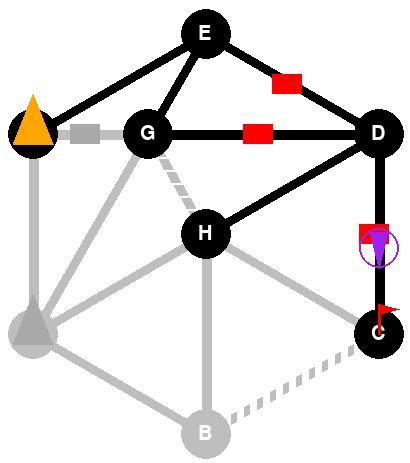
\includegraphics[width=0.75\textwidth]{assets/informatik-prototyp/simulator/sim-ui.png}
\caption{GUI des Simulators}
\label{fig:sim-gui}
\end{figure}

TODO BILD: Roboter auf Kante, mit entfernten Kanten 

\textbf{Trial and Error Mode}

Es wurde ein Modus implementiert, zu dem gewechselt wird, falls der Roboter nicht mehr weiss, wo er sich befindet. Dies soll im richtigen Roboter als Risikomitigation implementiert sein. Fuer die Simulation wurde ein Ablauf definiert fuer diesen Modus und er wurde implementiert. Die Nachrichten der Sensoren wurden gemockt.

\begin{figure}[H]
\centering
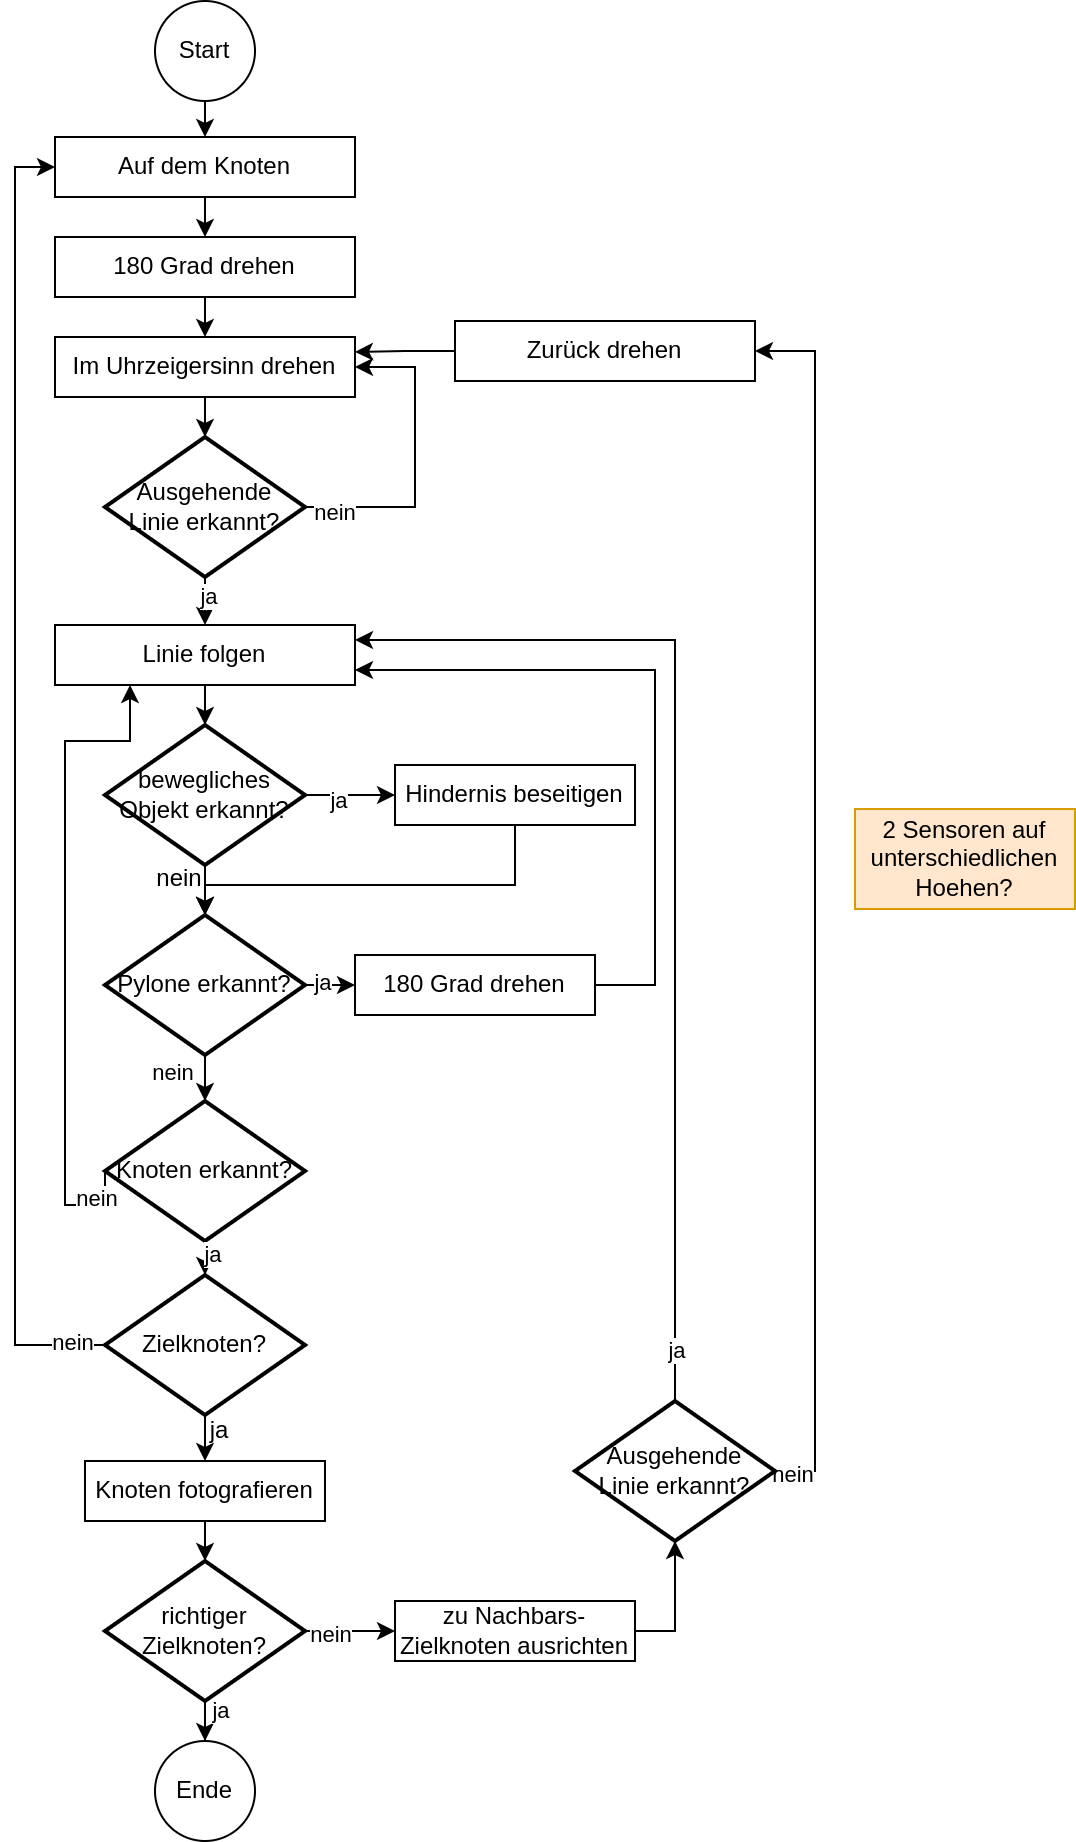
\includegraphics[width=0.75\textwidth]{assets/informatik-prototyp/simulator/simulator-trial-and-error-mode.png}
\caption{Trial and Error Mode}
\label{fig:sim-trial-error}
\end{figure}